\subsection{Módulo Alumnos}

  \paragraph{}El diagrama de la figura
  \ref{diagramaDescomposicionAlumnos} representa el módulo Alumnos. En primer
  lugar, el usuario alumno debe validar sus datos de acceso para que se permita
  o no el acceso a las funciones de las que se compone el módulo.

  \paragraph{}Desde este módulo, el alumno podrá acceder a todos los procesos
  necesarios para organizar correctamente toda su información personal, así
  como listar las reuniones en las que participe y su historial de asesores.

  \paragraph{}Además cuenta con un módulo de ayuda disponible en todo momento
  para el correcto manejo de la aplicación.

  \begin{figure}[!ht]
    \begin{center}
      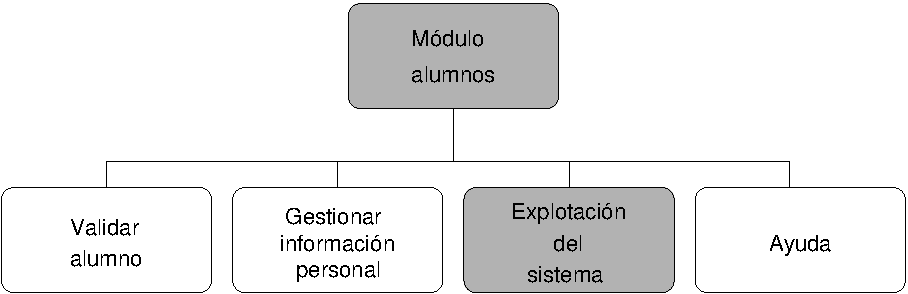
\includegraphics[]{11.Disenyo_Arquitectonico/11.2.Diagramas_Descomposicion/11.2.5.Modulo_alumnos/Diagramas/alumnos.pdf}
      \caption{Diagrama de descomposición del módulo Alumnos.}
      \label{diagramaDescomposicionAlumnos}
    \end{center}
  \end{figure}

% \paragraph{}El usuario administrador principal puede realizar consultas sobre
los centros, departamentos, titulaciones, asignaturas, usuarios y sobre
las plantillas oficiales que existan en el sistema. Además también puede
realizar consultar de datos históricos referentes a esta misma información en
diferentes cursos académicos.

\paragraph{}La figura \ref{diagramaNivel3-ExplotacionSistema-adminPrincipal}
muestra el nivel de abstracción 3: Explotación del sistema (módulo Administrador
principal).

  \begin{figure}[!ht]
    \begin{center}
      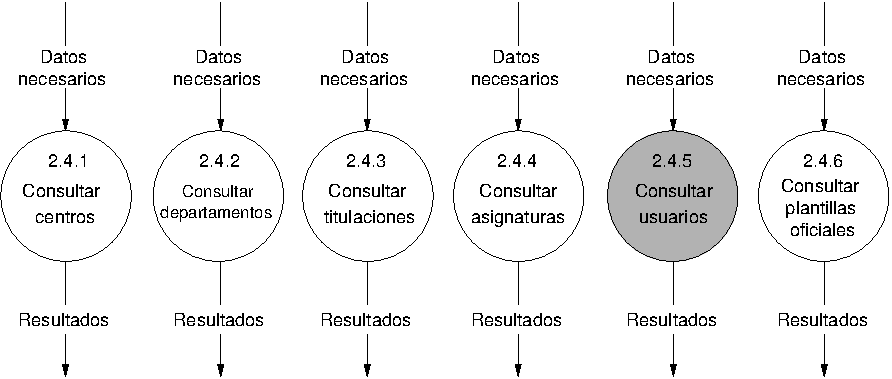
\includegraphics[]{08.Analisis_Funcional/8.2.DFDs/Niveles/Nivel3/AdministradorPrincipal/ExplotacionSistema/Diagramas/nivel3-ExplotacionSistema.pdf}
      \caption{Nivel de abstracción 3: Explotación del sistema (módulo
      Administrador principal).}
      \label{diagramaNivel3-ExplotacionSistema-adminPrincipal}
    \end{center}
  \end{figure}